\documentclass[../main/main.tex]{subfiles}

\newdate{date}{16}{10}{2019}

\begin{document}


\section{Thermodynamic of phase coexistence}

\subsection{Lever Rule}

\marginpar{ \textbf{Lecture 3.} \\  \displaydate{date}. \\ Compiled:  \today.}

The lever rule \cite{3_lesson_1} is a rule used to determine the mole fraction of each phase of a binary equilibrium phase diagram. For instance, it can be used to determine the fraction of liquid and solid phases for a given binary composition and temperature that is between the liquid and solid line.

In an alloy or a mixture with two phases, \( \alpha  \)  and \( \beta  \), which themselves contain two elements, \emph{A}  and \emph{B}, the lever rule states that the mass fraction of the \( \alpha  \)  phase is

\begin{equation}
w^{\alpha } = \frac{w_B - w_B^\beta }{w_B^\alpha - w_B^\beta }
\end{equation}
where
\begin{itemize}
\item \( w_B^\alpha  \):  is the mass fraction of element \emph{B}  in the \( \alpha  \) phase.
\item \( w_B^\beta   \):  is the mass fraction of element \emph{B} in the \( \beta  \)  phase.
\item \( w_B  \):  is the mass fraction of element \emph{B} in the entire alloy or mixture.
\end{itemize}

\begin{example}{}{}
  Consider Figure \ref{fig:3_0}; at all points between \emph{A} and \emph{B} the system is a mixture of gas and liquid. Points \emph{D} has global density \( \rho_D = \rho_A + \rho_B \)  and therefore \( v_D = \frac{1}{\rho_D}, v_A = \frac{1}{\rho _A}, v_B = \frac{1}{\rho_B} \) which implies:
  \begin{equation*}
    v_D = \frac{N_A}{N} v_A + \frac{N_B}{N} v_B = x_A v_A + x_B v_B
    \label{eq:}
  \end{equation*}
  Since \( x_A + x_B = 1 \) we have \( (x_A + x_B)v_D = x_A v_A + x_B v_B \) and finally by rearranging, one finds the \textit{Lever Rule}. It shows that the relative concentration of the liquid-gas mixture changes with \emph{V}:

  \begin{equation*}
    \frac{x_A}{x_B} = \frac{v_B - v_D}{v_D - v_A}
    \label{eq:}
  \end{equation*}
  
\end{example}

  \begin{figure}[h!]
  \centering
  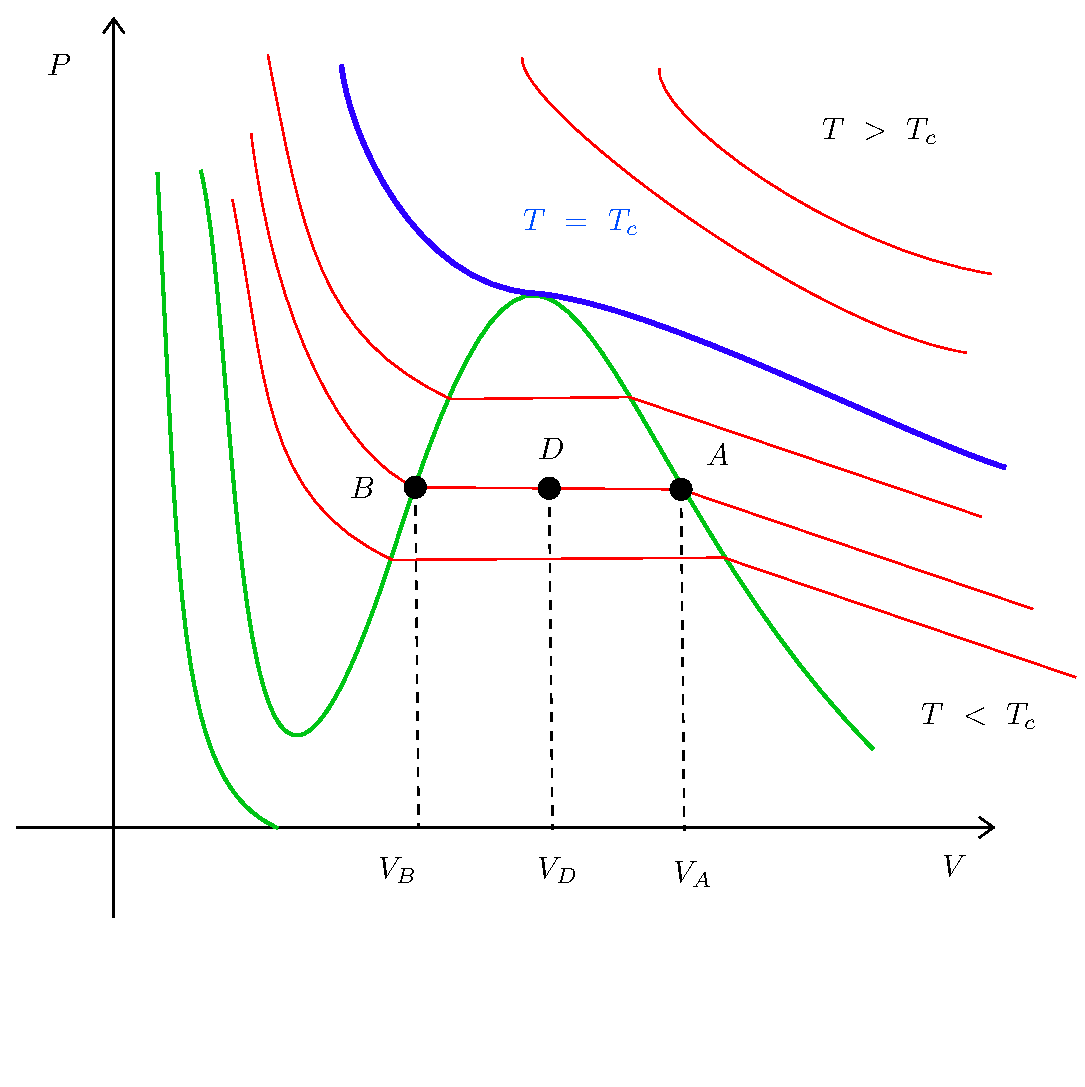
\includegraphics[width=0.6\textwidth]{../lessons/3_image/1.pdf}
  \caption{\label{fig:3_0} \( (V,P) \) projection. In the region between \emph{A} and \emph{B} the gas and the liquid phase coexist by keeping the pressure constant.}
  \end{figure}


\subsection{Phase coexistence (one component system)}

Consider a \( (P,V,T) \) system as a mixture of two species \( (1,2) \) at temperature \( T_1, T_2 \), pressure \( P_1, P_2 \) and chemical potentials \( \mu _1,\mu _2 \). The equilibrium condition is given by the maximum of the total entropy \( S = S_1 + S_2 \) and gives the conditions
\begin{equation}
  T_1 = T_2, \quad P_1 = P_2, \quad \mu _1 = \mu _2
  \label{eq:}
\end{equation}
this is the \emph{coexistence condition} of the two phases.

In terms of the Gibbs potential \( G = U- TS+PV \), where \emph{U} is given by  the Euler equation \( U = TS-PV+ \mu _1 N_1 + \mu _2 N_2 \), the Gibbs per mole is
\begin{subequations}
\begin{align}
  g_1 (T,P) &\equiv \frac{G_1}{N_1} = \mu _1 \\
  g_2 (T,P) &\equiv \frac{G_2}{N_2} = \mu _2
\end{align}
\label{}
\end{subequations}
Therefore, on the coexistence line it should hold the relation
\begin{equation}
  g_1 (T,P) = g_2 (T,P)
  \label{eq:}
\end{equation}

\subsection{Clausius-Clapeyron equation}
The coexistence curves \cite{3_lesson_2}, as the one illustrated in Figure  \ref{fig:3_1}, are less arbitrary than is immediately evident; the slope \( \dd[]{P} /\dd[]{T}   \) of a coexistence curve is fully determined by the properties of the two coexisting phases.

The slope of a coexistence curve is of direct physical interest. Consider cubes of ice at equilibrium in a glass of water. Given the ambient pressure, the temperature of the mixed system is determined by the liquid-solid coexistence curve of water; if the temperature were not on the coexistence curve some ice would melt, or some liquid would freeze, until the temperature would again lie on the coexistence curve (or one phases would become depleted). If the ambient pressure were to decrease perhaps, by virtue of a change in altitude, then the temperature of the glass of water would appropriately adjust to a new point on the coexistence curve. If \( \Delta P \) were the change in pressure, then the change in temperature would be \( \Delta T = \Delta P / (\dd[]{P} /\dd[]{T})_{coex} \), where the derivative in the denominator is the slope of the coexistence curve.

\begin{remark}
Ice skating presents another interesting example. The pressure applied to the ice directly beneath the blade of the skate shifts the ice across the solid-liquid coexistence curve, providing a lubricating film of liquid on which the skate slides. The possibility of ice skating depends on the negative slope of the liquid-solid coexistence curve of water.
\end{remark}
\begin{figure}[h!]
\centering
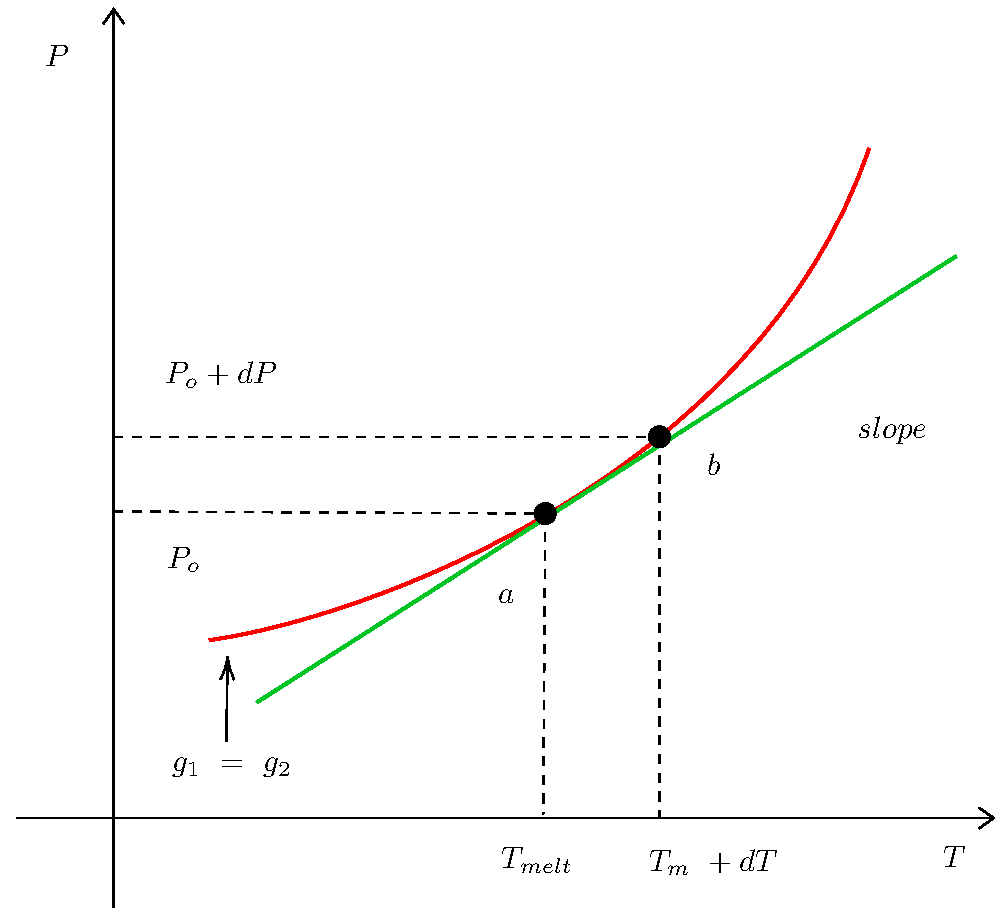
\includegraphics[width=0.7\textwidth]{../lessons/3_image/2.pdf}
\caption{\label{fig:3_1} \( (T,P) \) projection. The coexistence line is represented in red, while in green the slope between the two points \emph{a} and \emph{b}.}
\end{figure}

Now, suppose to know the position on the coexistence line (for example the melt temperature \( T_m \) at the atmospheric pressure \( P_0 \)). Is it possible to find other points on the curve? For example \( T_m \) at lower or higher pressure?


The answer is yes for small deviations of \emph{T} and \emph{P} from \emph{a}. The idea is to compute the slope of the tangent of the coexistence curve, i.e. \( (\dd[]{P}/\dd[]{T}  )  \). This is given by the Clausius-Clapeyron equation.
Both at \emph{a} and \emph{b} the two phases 1 and 2 coexist. This means  that at the coexistence line
\begin{equation}
  \begin{cases}
   g_1^{(a)} = g_2^{(a)}\\
   g_1^{(b)} = g_2^{(b)}
  \end{cases}
\label{eq:}
\end{equation}
Hence, if \emph{a} and \emph{b} are very close:
\begin{equation}
  \begin{cases}
  \dd[]{g_1} = g_1^{(b)} - g_1^{(a)} \\
  \dd[]{g_2} = g_2^{(b)} - g_2^{(a)}
  \end{cases}
\label{eq:}
\end{equation}
Therefore, the \emph{starting point} for \emph{Clausius-Clapeyron} is
\begin{equation}
  \Rightarrow \dd[]{g_1} =\dd[]{g_2}
  \label{eq:}
\end{equation}
From the molar version of the Gibbs-Duhem relation, we have
\begin{equation}
  \begin{cases}
   \dd[]{g_1} = -s_1 \dd[]{T} + v_1 \dd[]{P} = \dd[]{\mu _1}    \\
   \dd[]{g_2} = -s_2 \dd[]{T} + v_2 \dd[]{P} = \dd[]{\mu _2}
  \end{cases}
\label{eq:}
\end{equation}
taking the difference, one obtains
\begin{equation*}
  -(s_2 - s_1) \dd[]{T} + (v_2 - v_1) \dd[]{P} = 0
\end{equation*}
The slope is called \textbf{Clausius-Clapeyron equation}:
\begin{empheq}[box=\myyellowbox]{equation}
  \qty(\dv{P}{T} )_{coex} = \frac{(s_2-s_1)}{(v_2-v_1)} = \frac{\Delta s}{\Delta v}
\end{empheq}
\begin{remark}
Since \( (\dd[]{P}/\dd[]{T})_{coex}   \) is finite, the equation explains why a first order transition is characterised by discontinuous changes in entropy and volume (or density). \( \Delta S \)  gives the latent heat \( L_{12} \) \footnote{The latent heat of fusion is the quantity of heat required to melt one mole of solid.}:
\begin{equation}
  L_{12} = T \Delta s
\end{equation}
whence, the Clapeyron equation is
\begin{equation}
  \dv{P}{T}  = \frac{L_{12}}{T \Delta v}
\end{equation}
\end{remark}


\subsection{Application of C-C equation to the liquid-gas coexistence line}
\begin{figure}[h!]
\centering
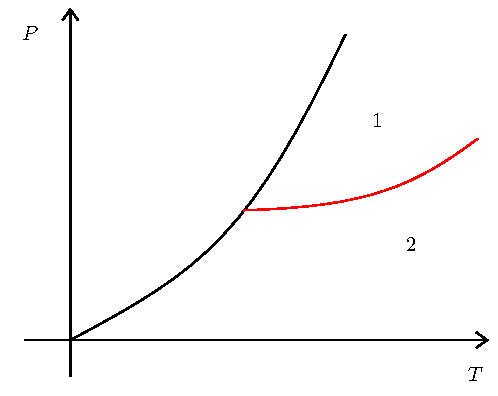
\includegraphics[width=0.5\textwidth]{../lessons/3_image/16.pdf}
\caption{\label{fig:3_16} \( (T,P) \) projection. Region 1: liquid. Region 2: gas. The lines represent the combinations of pressures and temperatures at which two phases can exist in equilibrium.}
\end{figure}

 Now, we go from gas (region 2) to liquid (region 1), we have:
\begin{equation*}
  \qty(\dv{P}{T} )_{coex} = \frac{s_2 - s_1}{v_2 - v_1}
  \label{eq:}
\end{equation*}

The Clapeyron equation embodies the \emph{Le Chatelier principle}\footnote{"When a settled system is disturbed, it will adjust to diminish the change that has been made to it".}.
 Consider a liquid-gas transition (the coexistence curves, from which the inequality sign is derived, are shown in Figure \ref{fig:3_16}):
\begin{equation*}
  \qty(\dv{P}{T} )_{coex} > 0 \quad \Rightarrow \frac{s_2 - s_1}{v_2 - v_1} > 0
\end{equation*}
and since \( v_2 > v_1 \), we have \( s_2 > s_1 \). The gas has more entropy as it should be.  The slope of the phase curve is positive, then an increase in pressure at constant temperature tends to drive the system to the more dense (solid) phase, and an increase in temperature tends to drive the system to the more entropic (liquid) phase.


When going from a low-temperature phase to a high-temperature phase entropy always increases \( \Delta S > 0 \), because \( c_P \equiv T (\partial{S}/\partial{T}  )_P > 0 \).

The sign of \( \Delta V \) is more uncertain though. To see this point, let us consider the C-C equation at the solid-liquid (now solid is region 1 and liquid region 2) coexistence curve.
At the melt temperature:
\begin{equation*}
  \qty(\dv{P}{T} )_{coex} = \frac{\delta Q_{melt}}{T_{melt}\Delta v_{melt}}, \qquad \delta Q_{melt} = Q_{liq} - Q_{solid} > 0
  \label{eq:}
\end{equation*}
In general, \( \Delta v_m = v_{liq} - v_{solid} > 0 \) which implies \( \qty( \dd[]{P}/\dd[]{T}   )_{coex} > 0  \). There are cases, however, where \( \Delta v_m = v_{liq} - v_{solid} < 0 \) because \( \rho_{liq} > \rho _{solid} \) (for instance the \( H_2 0 \), or also Silicon and Germanium). The paradigmatic example is the freezing of water where \( v_{ice} > v_{liq} \) since ice is less dense than liquid water at the coxistence (\( 0 < T° < 4 \)). This implies that \( \dd[]{P}/\dd[]{T} < 0   \).

\begin{example}{Melting point on Everest}{}

Consider \( T = 237 K \) and \( P=P_0 \). If we suppose that
\begin{equation*}
\delta Q_m = 6.01 kJ/mol, \quad \Delta v = -1.7 cm^3 /mol    
\end{equation*}
we have
\begin{equation*}
  \dv{P}{T}  = \frac{\delta Q_m}{T \Delta v} = \frac{6.01 10^3 J/mol}{273 \cdot (-1.7 cm^3/mol)} = -1.29 \cdot 10^4 J/m^3 = -1.29 bar/K
  \label{eq:}
\end{equation*}
\begin{equation*}
  \Rightarrow \Delta T = \frac{\Delta P}{(-1.29 Pa/K)} = \frac{(P_0 - P_{\text{Everest}})}{(-1.29 Pa/K)} = \frac{(1-0.36)atm}{(-1.29 Pa/K)} = -0.5\SI{}{\celsius}
  \label{eq:}
\end{equation*}
\begin{equation*}
  \Rightarrow T_m ( \text{Everest}) = T_m (P_0) + 0.5\SI{}{\celsius}
  \label{eq:}
\end{equation*}
\end{example}

\begin{example}{Boiling point on Everest}{}

Let us consider
\begin{equation*}
 P_{\text{Everest}}= 0.36 atm, \quad \rho (T= 100\SI{}{\celsius})=0.598 kg/m^3, \quad
  L_{gl} = 2.257 \cdot 10^3 J/g
\end{equation*}
The density of the vapour (gas) is about 1000 less than water (liquid), it implies that: 
\begin{equation*}
 \Delta V = V_g - V_l \approx V_g = \frac{1}{\rho_g}   
\end{equation*}
 We have:
\begin{equation*}
  \dv{P}{T} = \frac{L_{ge}}{T \Delta V} = \frac{L_{ge} \rho _g}{T} = \frac{2.25 \cdot 10^3 J/g \cdot 0.593 kg/m^3}{373 K} = \frac{3.6}{K} \frac{10^3 J}{g} \frac{kg}{m^3} = 3.6 \cdot 10^3 \frac{Pa}{K} 
\end{equation*}
\begin{equation*}
  \Rightarrow \Delta T \approx \Delta P/(3.6 10^3 Pa/K) = 18 \SI{}{\celsius}   
  \label{eq:}
\end{equation*}
\begin{equation*}
 \Rightarrow T_0 - T_{\text{Everest}} = 18\SI{}{\celsius} \quad \Rightarrow T_{\text{Everest}}\approx 80\SI{}{\celsius}   
\end{equation*}
\end{example}

\section{Order parameter of a phase transition}
An order parameter is a measure of the degree of order across the boundaries in a phase transition system. In particular,
 \emph{order parameters} are macroscopic observable that are equal to zero above the critical temperature, and different from zero below:

 \begin{empheq}[box=\myyellowbox]{equation}
   O_p =
     \begin{cases}
     \neq 0 & T<T_c \\
     = 0 & T \rightarrow T_c^-
     \end{cases}
 \end{empheq}
When a phase transition implies a breaking of a phase symmetry, the order parameter is related to this symmetry. Therefore, the order parameter reflects the symmetry of the system. Recall that, at \( T_c \) the system has a symmetry broken.


For instance, consider the densities of liquid and gas and the related order parameter of the gas-liquid transition \( \Delta \rho = \rho _{l} - \rho _{g} \), that is \( \neq 0 \) for \( T \neq T_c \) but \( \rightarrow 0 \) when \( T \rightarrow T_c \) (see Figure \ref{fig:3_2}).

\begin{figure}[h!]
\centering
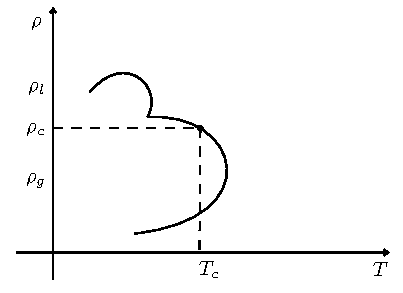
\includegraphics[width=0.6\textwidth]{../lessons/3_image/3.pdf}
\caption{\label{fig:3_2} \( (T,\rho ) \) projection of the \( (P,V,T) \) system, where \( \rho = N/V \). }
\end{figure}

\begin{remark}
Note that \( \rho = \frac{N}{V} = \frac{1}{v} \) hence either \emph{N} or \emph{V} varies.
\end{remark}


In Figure \ref{fig:3_3} is shown the behaviour for a ferromagnetic system. We have 
\begin{equation*}
  H= 0 \Rightarrow \begin{cases}
    M \neq 0 & T < T_c   \\
    M \rightarrow 0 & T \rightarrow T_c^-
\end{cases}
\end{equation*}
Clearly \( M \neq 0 \) if \( H \neq 0 \). Recall that \emph{M} is the order parameter of the paramagnetic-ferromagnetic phase transition. 
\begin{figure}[h!]
\centering
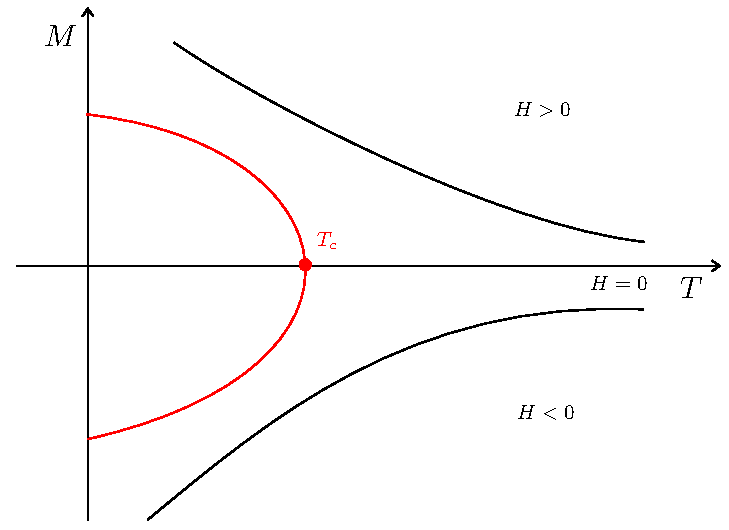
\includegraphics[width=0.7\textwidth]{../lessons/3_image/5.pdf}
\caption{\label{fig:3_3} Magnetization of a ferromagnet. In red: zero-field magnetization. Below the critical temperature there is a spontaneous magnetization.}
\end{figure}


It can be either a scalar ($\Delta \rho$), a vector ($\Vec{M}$) or even tensor ($Q_{\alpha \beta}$).
\subsubsection{Variable conjugate to \( O_P \)}
\begin{itemize}
\item \emph{Ferromagnetic system}: \( \va{M} \rightarrow \va{H}   \) (magnetic field).
\item \emph{Ferroelectric}: \( \va{P} \rightarrow \va{E}   \)  (electric field).
\item \emph{Liquid crystals}: \( Q_{\alpha \beta } \rightarrow \va{E},\va{H}   \).
\item \emph{Fluid}: \( V \rightarrow P \) (pressure), or \( \rho \rightarrow \mu  \).
\end{itemize}









\section{Classification of the phase transitions}

\subsection{Thermodynamic classification}
Thermodynamically, one can distinguish two kinds of phase transitions:
\begin{enumerate}
\item Ones who develop latent heat.
\item Ones who do not develop latent heat. The entropy changes continuously at the transition.
\end{enumerate}
\subsection{Eherenfest classification}
The \emph{Eherenfest classification} is based on the behaviour of the derivatives of the thermodynamic potentials.

A phase transition is of order \emph{n} if all the \( (n-1) \)  derivatives are continuous and the \( n^{th} \) derivative displays a finite discontinuity.

\begin{example}{}{}
For instance, a first order transition in which \( S=-(\partial{G}/\partial{T}  )_P \) has finite discontinuity.
\end{example}
\begin{remark}
There are first order transitions where \emph{S} is continuous (no latent heat), but \( \rho  \) is discontinuous (\( v = (\partial{G}/\partial{P}  )_T \)).
\end{remark}
\begin{example}{}{}
Second order transition. The specific heat displays a finite jump, see Figure \ref{fig:3_04_3} in the conductor-superconductor transition.

Another example is a second order transition but with divergence. Consider the fluid-superfluid transition (or \( \lambda  \) transition) of the \( \text{He}_4 \) (Figure \ref{fig:3_04_4}).
\end{example}



\begin{figure}[h!]
\begin{minipage}[c]{0.5\linewidth}
\centering
\subfloat[][]{
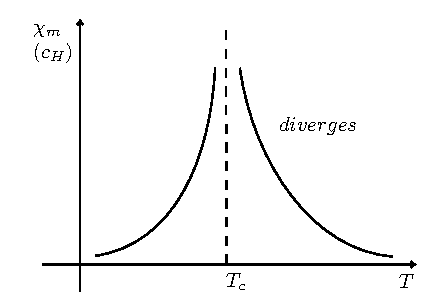
\includegraphics[width=1\textwidth]{../lessons/3_image/6.pdf}
    \label{fig:} }
\end{minipage}
\begin{minipage}[]{0.5\linewidth}
\centering
\subfloat[][Liquid gas \( k_T = - \frac{1}{V} \pdv{V}{P}  \) ]{
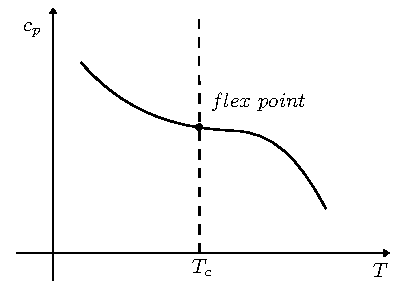
\includegraphics[width=1\textwidth]{../lessons/3_image/7.pdf}
    \label{fig:} }
\end{minipage}
\\
\begin{minipage}[c]{0.5\linewidth}
\centering
\subfloat[][2° order phase transition]{
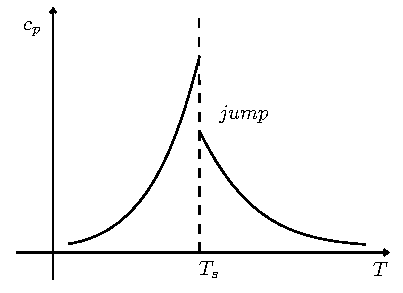
\includegraphics[width=1\textwidth]{../lessons/3_image/8.pdf}

    \label{fig:3_04_3} }
\end{minipage}
\begin{minipage}[]{0.5\linewidth}
\centering
\subfloat[][Superfluid in \( \lambda\)-transition ]{
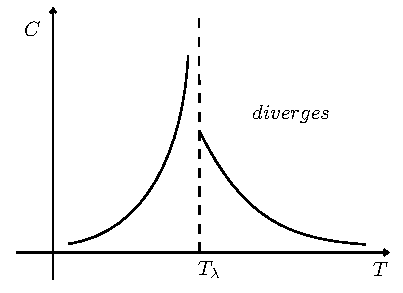
\includegraphics[width=1\textwidth]{../lessons/3_image/9.pdf}
    \label{fig:3_04_4} }
\end{minipage}
\caption{\label{fig:} Plots of response functions.}
\end{figure}

\begin{remark}
\( \lambda  \) transition: a second-order or higher-order transition, in which the heat capacity shows either a discontinuity (second-order) or a vertex (higher-order) at the transition temperature.  It is so named because the shape of the specific heat versus temperature curve resembles the Greek letter \( \lambda  \).
\end{remark}

\subsection{Modern classification}
A phase transition is of the first order if exists a finite discontinuity in either one or more partial derivatives of the thermodynamic potentials. Instead, if the first derivatives are all continuous, but the second are either discontinuous, or infinite, one talks of continuous transitions.
A critical point is a continuous transition.




\section{Critical exponents}

At the critical point response functions may diverge. How are these divergence?
In general, when you are close to \( T_c \), there are singolarities. Now, we can ask, how the curve diverges? What is the behaviour close to the critical point? Power law, so which are the values of these critical exponents?

\subsection{Divergence of the response functions at the critical point}
\label{sec:3_1}
While at the critical point the order parameter goes to zero continuously as \( T \rightarrow T_c^- \), the response function may develop divergences.
\begin{example}{}{}
In a fluid system since at \( T=T_c \) the curve \( P = P(V) \) develops an horizontal flex (Figure \ref{fig:3_2_2}), we have \( k_T = -\frac{1}{V} \qty(\pdv{V}{P} )_T  \rightarrow \infty  \). Similarly, in a magnetic since the curve is like Figure \ref{fig:3_3}, we have \( \chi _T = \qty(\pdv{M}{H} )_T \underset{T \rightarrow  T_c}{\rightarrow } \infty   \).

\end{example}

\begin{figure}[h!]
\centering
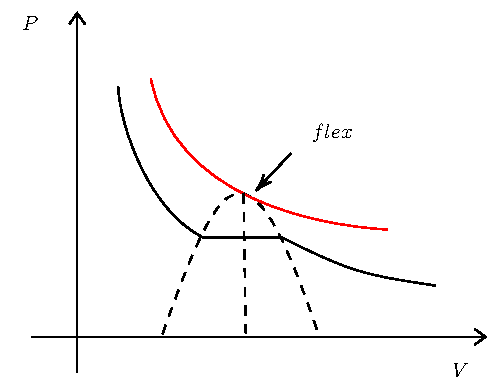
\includegraphics[width=0.5\textwidth]{../lessons/3_image/4.pdf}
\caption{\label{fig:3_2_2} \( (V,T) \) projection.  }
\end{figure}


\subsection{Critical exponents definition}

The notion of \emph{critical exponent} describes the behaviour of the order parameter and the response functions in proximity of the critical point.
In order to answer to these questions, let us define:


\begin{definition}{Critical Exponent, \emph{or} Scale Exponent}{}
Let us define the adimensional parameter measuring the distance from the critical point \( t \equiv \frac{T-T_c}{T_c} \), the \emph{critical exponent} \( \lambda  \) associated to the function \( F(t) \) is defined as:
\begin{equation}
  \lambda _{\pm} = \lim_{t \rightarrow 0^{\pm}} \frac{\ln{\abs{F(t)} } }{\ln{\abs{t} } }
\end{equation}
\end{definition}

We note that it behaves like a power law. One can also write the \textit{power law}:
\begin{equation}
  F(t) \overset{t \rightarrow  0^{\pm}}{\sim } \abs{t}^{\lambda _{\pm}}
\end{equation}
More generally, for \( t \ll 1 \):
\begin{equation}
  F(t) = A \abs{t}^{\lambda _{\pm}} ( 1 + bt^{\lambda _1}+ \dots), \quad \lambda _1 > 0
\end{equation}
where all other terms are less important.

\begin{definition}{Thermodynamic Critical Exponents}{}
\begin{itemize}
\item \textbf{Exponent \( \pmb{\beta} \)}: tells how the order parameter goes to zero.
Consider Figure \ref{fig:3_4_1}, we have \( \abs{M} \overset{t \rightarrow  0^-}{\sim} (-t)^{\beta }  \). No sense in going from above \( (t \rightarrow 0^+) \) where it stays 0.

\item \textbf{Exponent \(\pmb{ \gamma _{\pm} } \)} (susceptibility): related to the response function. Consider Figure \ref{fig:3_4_2}, we have \( \chi _T \overset{t \rightarrow 0^{\pm}}{\sim} \abs{t}^{-\gamma _{\pm} }   \). In principle, the value of \( \gamma   \) can depend on the sign of \emph{t} i.e.   \( \gamma ^+ \neq \gamma ^-  \), but they are the same in reality and we have \( \gamma ^+ = \gamma ^- = \gamma     \).

\item \textbf{Exponent \(\pmb{ \alpha _{\pm} }\)}: how specific heat diverges (second order derivative in respect of \emph{T}). For instance see Figure \ref{fig:3_4_3}, we have \( c_H \sim \abs{t}^{-\alpha _{\pm}}  \).

\item \textbf{Exponent \( \pmb{\delta   }\)}: in this case one consider the isotherm \( T =T_c \) and look for the behaviour of \emph{M} at the critical point at small \emph{H} (or viceversa).  The result is \( M \sim H^{1/\delta } \).
In Figure \ref{fig:3_4_4}, \( H \sim \abs{M}^{\delta } \text{sign} (M)  \).

\end{itemize}
\end{definition}



\begin{figure}[h!]
\begin{minipage}[c]{0.5\linewidth}
\centering
\subfloat[][Exponent \( \beta  \).]{
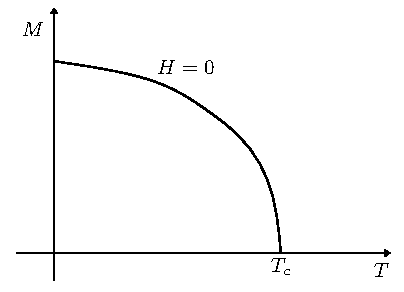
\includegraphics[width=1\textwidth]{../lessons/3_image/10.pdf}
    \label{fig:3_4_1} }
\end{minipage}
\begin{minipage}[]{0.5\linewidth}
\centering
\subfloat[][Exponent \( \gamma_{\pm}  \).]{
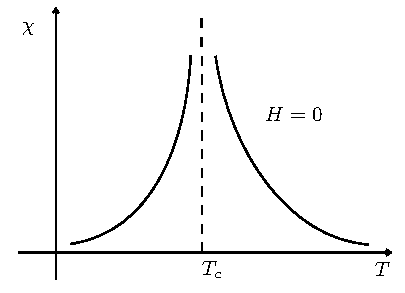
\includegraphics[width=1\textwidth]{../lessons/3_image/11.pdf}
    \label{fig:3_4_2} }
\end{minipage}
\\
\begin{minipage}[c]{0.5\linewidth}
\centering
\subfloat[][Exponent \( \alpha _{\pm} \).]{
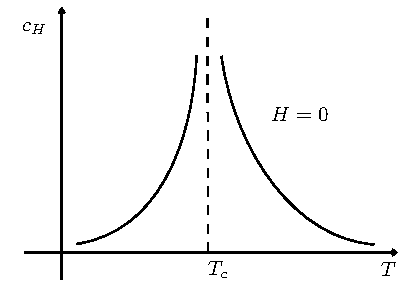
\includegraphics[width=1\textwidth]{../lessons/3_image/12.pdf}
    \label{fig:3_4_3} }
\end{minipage}
\begin{minipage}[]{0.5\linewidth}
\centering
\subfloat[][Exponent \( \delta   \).]{
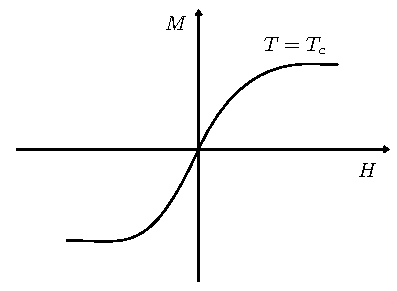
\includegraphics[width=1\textwidth]{../lessons/3_image/13.pdf}
    \label{fig:3_4_4} }
\end{minipage}
\caption{\label{fig:}}
\end{figure}


\begin{table}[h!]
  \begin{center}
\begin{tabular}{cc}
\toprule
 Zero-field specific heat & \( C_H \sim \abs{t}^{-\alpha }  \) \\
 Zero-field magnetization & \( M \sim (-t)^{\beta } \) \\
 Zero-field isothermal susceptibility & \( \chi _T \sim \abs{t}^{-\gamma  }  \) \\
 Critical isotherm \( (t=0) \) & \( H \sim \abs{M}^\delta \text{sign} (M)  \)  \\
 Correlation length & \( \xi \sim \abs{t}^{- \nu }  \) \\
 Pair correlation function at \( T_c \) & \( G (\va{r}) \sim \frac{1}{r^{d-2+ \eta }} \) \\
\bottomrule
\end{tabular}
\end{center}
\caption{\label{tab:3_1} Definitions of the most commonly used critical exponents for a magnetic system \cite{3_lesson_3}.}
\end{table}

\begin{table}[h!]
  \begin{center}
\begin{tabular}{cc}
\toprule
Specific heat at constant volume \( V_c \)  & \( C_V \sim \abs{t}^{-\alpha }  \) \\
Liquid-gas density difference & \( (\rho _l - \rho _g)\sim (-t)^{\beta } \) \\
Isothermal compressibility & \( k _T \sim \abs{t}^{-\gamma  }  \) \\
 Critical isotherm \( (t=0) \) & \( P-P_c \sim \abs{\rho _l - \rho _g}^\delta \text{sign} (\rho _l - \rho _g)  \)  \\
 Correlation length & \( \xi \sim \abs{t}^{- \nu }  \) \\
 Pair correlation function at \( T_c \) & \( G (\va{r}) \sim \frac{1}{r^{d-2+ \eta }} \) \\
\bottomrule
\end{tabular}
\end{center}
\caption{ \label{tab:3_2} Definitions of the most commonly used critical exponents for a fluid system \cite{3_lesson_3}.}
\end{table}

\begin{remark}
In compiling Table \ref{tab:3_1} and \ref{tab:3_2} we have made the as yet totally unjustified assumption that the critical exponent associated with a given thermodynamic variable is the same as \( T \rightarrow T_c \) from above or below.
\end{remark}

Critical exponents depend on very few parameters and are not system-specific:
1 - symmetries of the system
2 - dimension of the system
3 - range of interaction
$T_c$ instead does depend on specific chemistry, is not as universal as critical exponent.


\subsection{Law of the corresponding states}
The system displays correlation at very long distance, these goes to the size of the system when \( T \rightarrow T_c \). We are talking about long range correlation. The \emph{correlation function} is \( \xi \sim t^{-\nu } \).
For instance, consider a polymer as in Figure \ref{fig:3_5}.

Having defined the critical exponents, we need to justify why they are interesting and  why they are more interesting than the critical temperature \( T_c \) itself. It turns out that, whereas \( T_c \) depends sensitively on the details of the interatomic interactions, the critical exponents are to a large degree \emph{universal} depending only on a few fundamental parameters.

To summurize, the critical exponents are more interesting than \( T_c \) since their values do not depend on microscopic details, but only on few parameters such as the space dimension \emph{d} and the symmetry of the system.

One of the first experimental evidence of this universality was given by the work of Guggenheim on the coexistence curves of \emph{g} different fluids: A, Kn, $\chi_e$, Ne, $N_2$, $CO_2$ and $O_2$. By plotting \( T/T_c \) versus \( \rho /\rho _c \) (Figure \ref{fig:3_6}) he found that all the data collapse on the same curve, i.e. different sets of data fit the  same function. Moreover for \( t \rightarrow 0 \):
\begin{equation*}
  (\rho _l - \rho _c) \sim (-t)^{\beta}
  \label{eq:}
\end{equation*}
and \( \beta \sim 1/3 \approx 0.335 \).  Therefore, close to the critical point all the data lie on the same curve and hence can be described by the same exponent \( \beta  \).
A further test of universality is to compare this value to that obtained for a phase transition in a completely different system with a scalar order parameter. For instance, if we do the same for a string ferromagnetic the result is \( \beta = 1/3 \)  too.
\begin{remark}
The law of corresponding states gives a universal liquid-gas coexistence curve.
\end{remark}





\begin{figure}[h!]
\begin{minipage}[c]{0.5\linewidth}

\subfloat[][\emph{N}-Polymer.]{   \centering
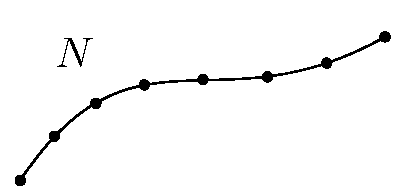
\includegraphics[width=1\textwidth]{../lessons/3_image/14.pdf}
    \label{fig:3_5} }
\end{minipage}
\begin{minipage}[]{0.5\linewidth}
\centering
\subfloat[][Coexistence curve of different fluids plotted in reduced variables.]{   \centering
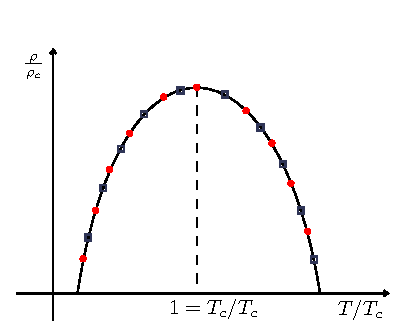
\includegraphics[width=1\textwidth]{../lessons/3_image/15.pdf}
    \label{fig:3_6} }
\end{minipage}
\caption{\label{fig:} }
\end{figure}


\subsection{Thermodynamic inequalities between critical exponents}
\label{sec:3_2}
It is possible to obtain several rigorous inequalities between the critical exponents. The easiest to prove is due to Rushbrooke.
\subsubsection{Rushbrocke inequality}
It follows from the well known thermodynamic relation between the specific heats at constant field and constant magnetization.
Remember the relation between response functions:
For a fluid:
\begin{equation*}
   k_T (c_p-c_v)=T v \alpha ^2 = T v \frac{1}{v^2} \qty(\pdv{v}{T} )^2_P = T \frac{1}{v} \qty(\pdv{v}{T} )^2_P
\end{equation*}
For magnetic systems one has
\begin{equation*}
  \chi _T (c_H-c_M) = T \underbrace{ \qty(\pdv{M}{T} )^2_H }_{\geq 0}
\end{equation*}
From thermodynamic stability we have \( c_M \geq 0, c_H \geq 0, \chi _T \geq 0  \).
Hence, from the previous relation we have
\begin{equation*}
   c_H = \frac{T}{\chi _T} \qty(\pdv{M}{T} )^2_H + \underbrace{c_M}_{\ge0}
\end{equation*}
which implies
\begin{equation}
   c_H \ge \frac{T}{\chi _T} \qty(\pdv{M}{T} )^2_H 
   \label{eq:3_1}
\end{equation}
On the other hand, for \( T \rightarrow T_c^- \) \( (t \rightarrow 0^-) \) and \( H=0 \) (zero field) we have
\begin{equation*}
  \begin{cases}
   c_H \sim (-t)^{-\alpha }\\
   \chi _T \sim (-t)^{-\gamma  } \\
    M \sim (-t)^{\beta }
  \end{cases}
\end{equation*}
that implies
\begin{equation*}
 \qty( \pdv{M}{T})_{H=0} \sim (-t)^{\beta -1}    
\end{equation*}
Since the inequality \eqref{eq:3_1} is valid for all temperature \emph{T}, it follows that can only be obeyed if
\begin{equation*}
  B (T_c - T)^{-\alpha } \ge B' T \frac{[(T_c - T)^{\beta -1}]^2}{(T_c-T)^{-\gamma  }}
\end{equation*}
with \( B,B' > 0 \). Take the limit \( T \rightarrow T_c^- \), we have:
\begin{equation*}
  \lim_{T \rightarrow T_c^-} (T_c - T)^{2- \alpha - 2 \beta - \gamma  } \ge \frac{B' T}{B} > 0
\end{equation*}
Since the left hand side must be strictly greater than zero, we have the \textit{RushBrook inequality}:

\begin{empheq}[box=\myyellowbox]{equation}
\alpha + 2 \beta  + \gamma \geq 2
\end{empheq}

\subsubsection{Griffith inequality}
The \emph{Griffith inequality} is obtained from the convexity property (in \emph{T} and \emph{V}) of the Helmolds free energy and from \( A \sim t^{2- \alpha } \) (as $t \rightarrow 0^-$ deduced from $c_P = t^{-\alpha}$):

\begin{empheq}[box=\myyellowbox]{equation}
  \Rightarrow \alpha + \beta (1+\delta ) \ge 2
\end{empheq}


\subsubsection{}
We have introduced two very new ideas, universality and inequalities between the critical exponents, which appear to hold as equalities (see Sec.\ref{sec:19_1}).

In the intervening chapters, we look  at models of systems which undergo phase transitions and how to calculate their critical exponents and other properties.






























\end{document}
